\chapter{THIẾT KẾ TRỤC TRUYỀN ĐỘNG}
    \section*{5.0 THÔNG SỐ BAN ĐẦU CÁC TRỤC}
        \subsection{Trục I}
            \begin{itemize}
                \item Công suất: $P_{I} = 3.07 \, \mathrm{kW}$.
                \item Số vòng quay: $n_{I} = 720 \, \mathrm{vòng/phút}$.
                \item Momen xoắn: $T_{I} = 40.72 \, \mathrm{N.m}$.
            \end{itemize}
        \subsection{Trục II}
            \begin{itemize}
                \item Công suất: $P_{II} = 2.86 \, \mathrm{kW}$.
                \item Số vòng quay: $n_{II} = 360 \, \mathrm{vòng/phút}$.
                \item Momen xoắn: $T_{II} = 75.87 \, \mathrm{N.m}$.
            \end{itemize}
        \subsection{Trục III}
            \begin{itemize}
                \item Công suất: $P_{III} = 2.72 \, \mathrm{kW}$.
                \item Số vòng quay: $n_{III} = 72 \, \mathrm{vòng/phút}$.
                \item Momen xoắn: $T_{III} = 360.78 \, \mathrm{N.m}$.
            \end{itemize}
        \subsection{Trục IV}
            \begin{itemize}
                \item Công suất: $P_{IV} = 2.5 \, \mathrm{kW}$.
                \item Số vòng quay: $n_{IV} = 12 \, \mathrm{vòng/phút}$.
                \item Momen xoắn: $T_{IV} = 1989.58 \, \mathrm{N.m}$.
            \end{itemize}
    \section{THIẾT KẾ TRỤC SƠ BỘ}
        \subsection{Chọn vật liệu chế tạo trục và ứng suất cho phép}
            \hspace*{0.6cm}Chọn vật liệu chế tạo các trục là thép C45 có $\sigma_{b} = 850 \, \mathrm{MPA}, \sigma_{ch} = 580 \, \mathrm{MPA}$, ứng suất uốn cho phép $[\sigma] = 80 \, \mathrm{MPA}$, chọn sơ bộ ứng suất xoắn cho phép $[\tau] = 20 \, \mathrm{MPa}$. 
        
        \subsection{Xác định sơ bộ đường kính trục:}
            \begin{itemize}
                \item Đường kính trục động cơ điện:
                    \begin{align*}
                        d_{I} = (0.3 \div 0.35)a = (0.3 \div 0.35) \cdot 160 = (48 \div 56) \, \mathrm{mm}
                    \end{align*}
                    Theo tiêu chuẩn ta chọn $d_{I} = 50 \, \mathrm{mm}$
                \item Đường kính đầu trục vào của hộp giảm tốc:
                    \begin{align*}
                        d_{v} = (0.8 \div 1.2) \cdot d_{I} = (0.8 \div 1.2) \cdot 50 = (40 \div 60) \, \mathrm{mm}
                    \end{align*}
                    Theo tiêu chuẩn ta chọn $d_{v} = 50 \, \mathrm{mm}$
                \item Đường kính trục thứ II:
                    \begin{align*}
                        d_{II} \geq 10 \sqrt[3]{\frac{16T_{II}}{\pi \cdot [\tau]}} = 10 \sqrt[3]{\frac{16 \cdot 75.87}{\pi \cdot 20}} = 26.83 \, \mathrm{mm}
                    \end{align*}
                    Theo tiêu chuẩn ta chọn $d_{II} = 30 \, \mathrm{mm} \Rightarrow$ Chọn bề rộng ổ lăn $b_{0} = 16 \, \mathrm{mm}$.
                \item Đường kính trục thứ III
                    \begin{align*}
                        d_{III} \geq 10 \sqrt[3]{\frac{16T_{III}}{\pi \cdot [\tau]}} = 10 \sqrt[3]{\frac{16 \cdot 360.78}{\pi \cdot 20}} = 45.12 \, \mathrm{mm}
                    \end{align*}
                    Theo tiêu chuẩn ta chọn $d_{III} = 50 \, \mathrm{mm} \Rightarrow$ Chọn bề rộng ổ lăn $b_{0} = 27 \, \mathrm{mm}$.
                \item Đường kính trục thứ IV:
                    \begin{align*}
                        d_{IV} \geq 10 \sqrt[3]{\frac{16T_{IV}}{\pi \cdot [\tau]}} = 10 \sqrt[3]{\frac{16 \cdot 1989.58}{\pi \cdot 20}} = 79.72 \, \mathrm{mm}
                    \end{align*}
                    Theo tiêu chuẩn ta chọn $d_{IV} = 80 \, \mathrm{mm}$
            \end{itemize}
            \begin{figure}[H]
                \centering
                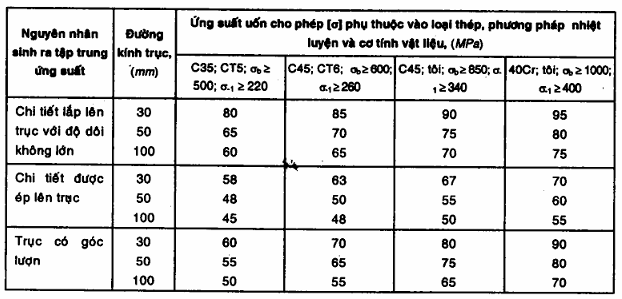
\includegraphics[width=0.8\textwidth]{pictures/bending_stress.png}
                \caption{Ứng suất uốn cho phép}
                \caption*{\footnotesize (Trích tài liệu \cite{gtctm}, trang 403, bảng 10.2)}
            \end{figure}
        \subsection{Chọn kích thước dọc trục}
            \begin{figure}[H]
                \centering
                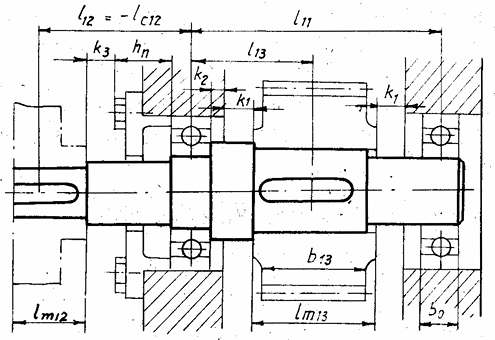
\includegraphics[width=0.75\textwidth]{pictures/shaft.png}
                \caption{Các kích thước dọc trục}
                \label{fig:shaft_standard}
            \end{figure} 
            \hspace*{0.6cm}Chọn các trị số của các thông số liên quan:
            \begin{itemize}
                \item [--] $k_1 = 10 \in (8 \div 15): $ Khoảng cách từ mặt mút của chi tiết quay đến thành trong của hộp.
                \item [--] $k_2 = 10 \in (5 \div 15): $ Khoảng cách từ mặt mút ổ đến thành trong của hộp.
                \item [--] $k_3 = 20 \in (10 \div 20): $ Khoảng cách từ mặt mút của chi tiết quay đến nắp ổ.
                \item [--] $h_n = 25 \in (15 \div 25): $ Chiều cao nắp ổ và đầu bu lông.
            \end{itemize}
            \subsubsection{Trục II}
                \begin{itemize}
                    \item Chiều rộng bánh đai:
                        $$l_{m12} = 44 (mm)$$   
                    \item Chiều dài đoạn $l_{12}$:
                        $$l_{12} = 0.5 \cdot (l_{m12} + b_0) + k_3 + h_n = 0.5 \cdot (44 + 16) + 20 + 25 = 75 (mm)$$
                    \item Chiều dài bánh răng trụ dẫn động:
                        $$l_{m13} = 53 (mm)$$
                    \item Chiều dài đoạn $l_{13}$:
                        $$l_{13} = 0.5 \cdot (l_{m13} + b_0) + k_1 + k_2 = 0.5 \cdot (53 + 16) + 10 + 10 = 54.5 (mm)$$
                    \item Chiều dài đoạn $l_{11}$:
                        $$l_{11} = 2 \cdot l_{13} + 10 = 119 (mm)$$
                    \item Chiều dài trục II:
                        $$l_{II} = l_{11} + l_{12} + 0.5 \cdot l_{m12} = 119 + 75 + 0.5 \cdot 44 = 216 (mm)$$
                \end{itemize}
            \subsubsection{Trục III}
                \begin{itemize}
                    \item Chiều rộng bánh răng côn dẫn động:
                        $$l_{m12} = 86.68 (mm)$$ 
                    \item Chiều dài đoạn $l_{12}$:
                        $$l_{12} = 0.5 \cdot (l_{m12} + b_0) + k_3 + h_n = 0.5 \cdot (86.68 + 29) + 15 + 20 = 92.84 (mm)$$
                    \item Chiều rộng bánh răng trụ bị dẫn:
                        $$l_{m13} = 48 (mm)$$ 
                    \item Chiều dài đoạn $l_{13}$:
                        $$l_{13} = 0.5 \cdot (l_{m13} + b_0) + k_1 + k_2 = 0.5 \cdot (48 + 29) + 10 + 10 = 58.5 (mm)$$
                    \item Chiều dài đoạn $l_{11}$:
                        $$l_{11} = 2 \cdot l_{13} + 16.5 = 133.5 (mm)$$
                    \item Chiều dài trục III:
                        $$l_{III} = l_{11} + l_{12} + 0.5 \cdot l_{m12} = 133.5 + 92.84 + 0.5 \cdot 86.68 = 269.68 (mm)$$
                \end{itemize}
        \subsection{Phân tích lực tác dụng lên trục}
            \subsubsection{Bánh đai bị dẫn}
                \begin{itemize}
                    \item Lực dọc trục bánh đai: $F_d = 813.8\, \mathrm{N}$.
                \end{itemize}
            \subsubsection{Bánh răng trụ 1}
                \begin{itemize}
                    \item Lực vòng bánh răng trụ 1: $F_{t1} = 2845.14 \, \mathrm{N}$.
                    \item Lực dọc trục bánh răng trụ 1: $F_{a1} = 870.39 \, \mathrm{N}$.
                    \item Lực hướng tâm bánh răng trụ 1: $F_{r1} = 1132.59 \, \mathrm{N}$. 
                \end{itemize}
            \subsubsection{Bánh răng trụ 2}
                \begin{itemize}
                    \item Lực vòng bánh răng trụ 2: $F_{t2} = 2845.11\, \mathrm{N}$.
                    \item Lực dọc trục bánh răng trụ 2: $F_{a2} = 870.39\, \mathrm{N}$.
                    \item Lực hướng tâm bánh răng trụ 2: $F_{r2} = 1132.59\, \mathrm{N}$. 
                \end{itemize}
            \subsubsection{Bánh răng côn 1}
                \begin{itemize}
                    \item Lực vòng bánh răng côn 1: $F_{t3} = 10091.75\, \mathrm{N}$.       
                    \item Lực dọc trục bánh răng côn 1: $F_{a3} = 603.71\, \mathrm{N}$.
                    \item Lực hướng tâm bánh răng côn 1: $F_{r3} = 3623.14\, \mathrm{N}$. 
                \end{itemize}
            \newpage
        \subsection{Vẽ biểu đồ momen uốn và xoắn}
            \subsubsection{Vẽ biểu đồ momen uốn và xoắn trục II}
                \begin{figure}[H]
                    \centering
                    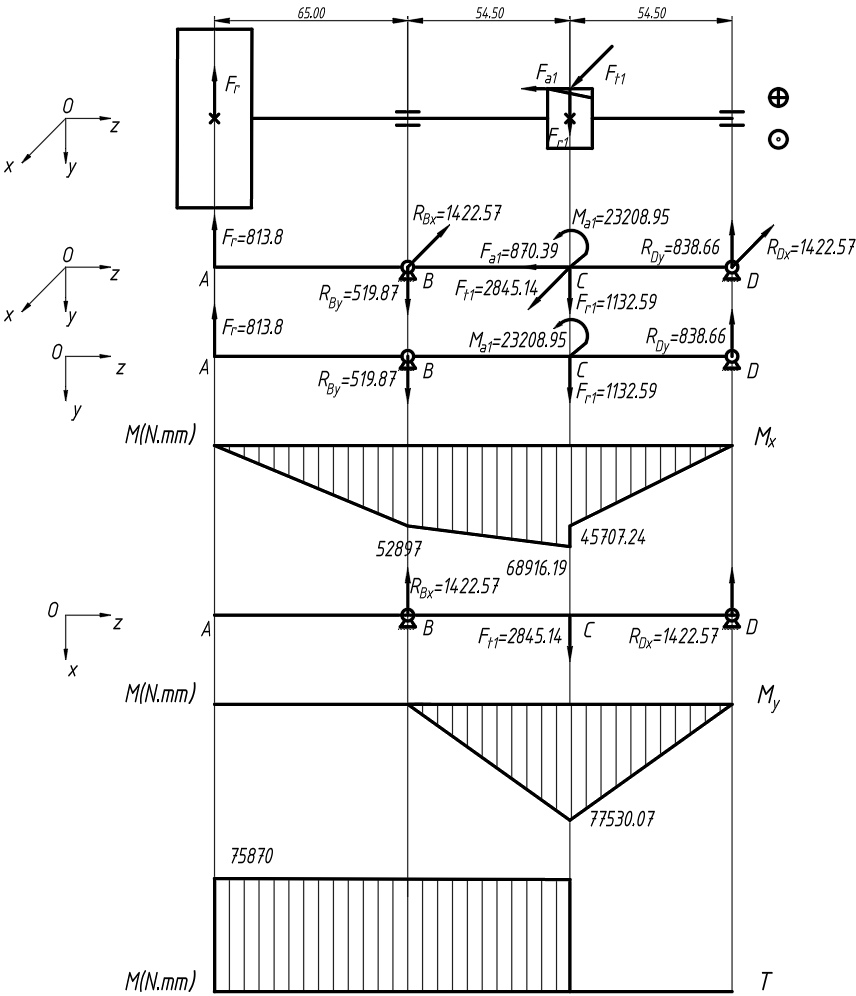
\includegraphics[width = 1\textwidth]{pictures/momen_II.png}
                    \caption{Biểu đồ momen trục II}
                    \label{fig:momen_II}
                \end{figure}
                \newpage
                \begin{itemize}
                    \item Biểu đồ momen uốn và xoắn như hình \ref{fig:momen_II}:
                    \item Trong mặt phẳng Oyz:
                        \begin{itemize}
                            \item Ta có phương trình cân bằng momen:
                            \begin{align*}
                                &\sum{M_{x/B}} = 0 \\
                                \Leftrightarrow& F_{r} \cdot 65 + F_{r1} \cdot 54.5 - M_{a1} - R_{Dy} \cdot 109 = 0 \\
                                \Leftrightarrow& F_{r} \cdot 65 + F_{r1} \cdot 54.5 - F_{a1} \cdot \frac{d_1}{2} - R_{Dy} \cdot 109 = 0 \\
                                \Leftrightarrow& R_{Dy} = \frac{813.8 \cdot 65 + 1132.59 \cdot 54.5 - 870.39 \cdot \frac{53.33}{2}}{109} = 838.66 \, \mathrm{N}
                            \end{align*}
                            \item Phương trình cân bằng lực theo trục y:
                            \begin{align*}
                                &\sum{F_{y}} = 0 \\
                                \Leftrightarrow& -F_{r} + R_{By} + F_{r1} - R_{Dy} = 0 \\
                                \Leftrightarrow& R_{By} = 838.66 + 813.8 - 1132.59 = 519.87\, \mathrm{N}
                            \end{align*}
                        \end{itemize}
                        \item Trong mặt phẳng Ozx:
                        \begin{itemize}
                            \item Ta có phương trình cân bằng momen:
                            \begin{align*}
                                &\sum{M_{y/B}} = 0 \\
                                \Leftrightarrow& F_{t1} \cdot 71 + R_{Dx} \cdot 132 = 0 \\
                                \Leftrightarrow& R_{Dx} = \frac{2845.11 \cdot 54.5}{109} = 1422.57 \, \mathrm{N}
                            \end{align*}
                            \item Phương trình cân bằng lực theo trục x:
                            \begin{align*}
                                &\sum{F_{x}} = 0 \\
                                \Leftrightarrow& -R_{Bx} + F_{t1} - R_{Dx} = 0 \\
                                \Leftrightarrow& R_{Bx} = 2845.11 - 1422.57 = 1422.57  \, \mathrm{N}
                            \end{align*}
                        \end{itemize}
                \end{itemize}
            \subsubsection{Vẽ biểu đồ momen uốn và xoắn trục III}
                \begin{figure}[H]
                    \centering
                    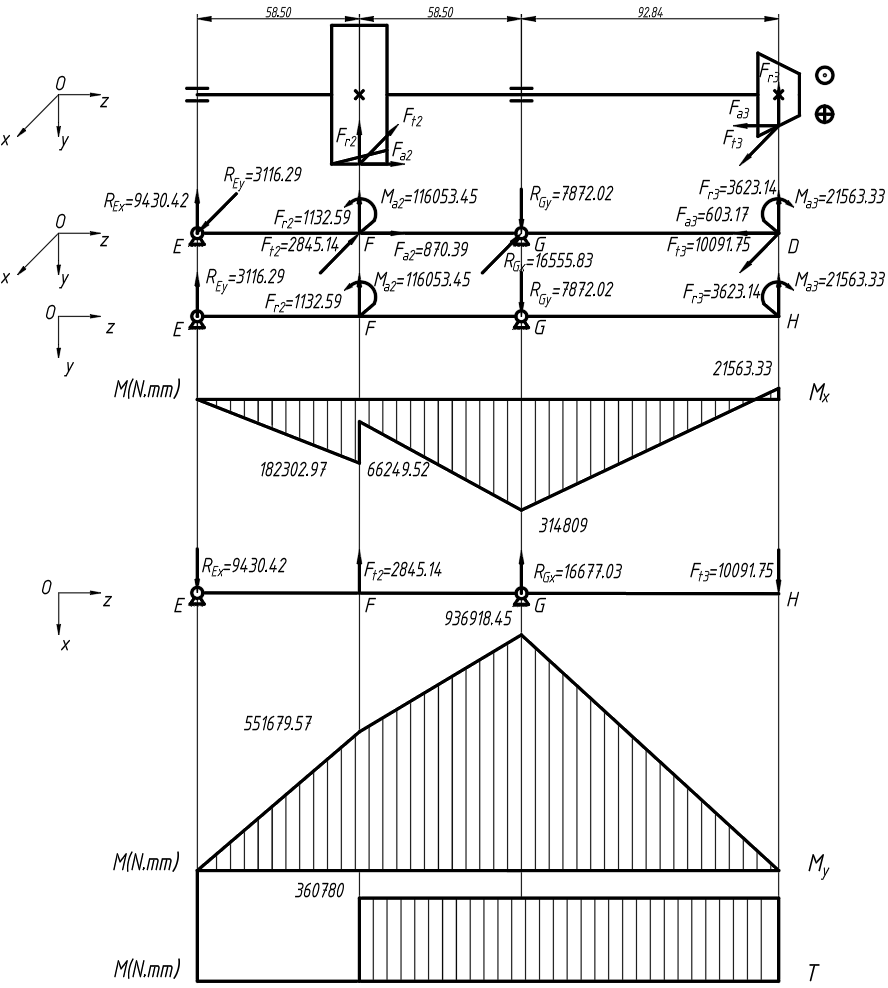
\includegraphics[width = 1.1\textwidth]{pictures/momen_III.png}
                    \caption{Biểu đồ momen trục III}
                    \label{fig:momen_III}
                \end{figure}
                \newpage
                \begin{itemize}
                    \item Biểu đồ momen uốn và xoắn như hình \ref{fig:momen_III}:
                    \item Trong mặt phẳng Oyz:
                        \begin{itemize}
                            \item Ta có phương trình cân bằng momen:
                                \begin{align*}
                                    &\sum{M_{x/E}} = 0 \\
                                    \Leftrightarrow& -F_{r2} \cdot 58.5 - M_{a2} + R_{Gy} \cdot 117 + M_{a3} - F_{r3} \cdot 224.84 = 0 \\
                                    \Leftrightarrow& -F_{r2} \cdot 58.5 - F_{a2} \cdot \frac{d_2}{2} + R_{Gy} \cdot 117 + F_{a3} \cdot \frac{d_3}{2} - F_{r3} \cdot 224.84 = 0 \\
                                    \Leftrightarrow& R_{Gy} = \frac{1132.59 \cdot 58.5 + 870.39 \cdot \frac{266.67}{2} - 603.17 \cdot \frac{71.5}{2} + 3623.14 \cdot 209.84}{117} = 7872.02 \, \mathrm{N}
                                \end{align*}
                            \item Phương trình cân bằng lực theo trục y:
                                \begin{align*}
                                    &\sum{F_{y}} = 0 \\
                                    \Leftrightarrow& R_{Ey} - F_{r2} + R_{Gy} - F_{r3} = 0 \\
                                    \Leftrightarrow& R_{Ey} = - 1132.59 - 3623.14 + 7872.02 = 3116.29 \, \mathrm{N}
                                \end{align*}
                        \end{itemize}
                    \item Trong mặt phẳng Ozx:
                        \begin{itemize}
                            \item Ta có phương trình cân bằng momen:
                                \begin{align*}
                                    &\sum{M_{y/E}} = 0 \\
                                    \Leftrightarrow& -F_{t2} \cdot 58.5 - R_{Gx} \cdot 117 + F_{t3} \cdot 224.84 = 0 \\
                                    \Leftrightarrow& -2845.14 \cdot 58.5 - R_{Gx} \cdot 117 + 10091.75 \cdot 224.84 = 0 \\
                                    \Leftrightarrow& R_{Gx} = \frac{-2845.14 \cdot 58.5 + 10091.75 \cdot 209.84}{117} = 16677.03\, \mathrm{N}
                                \end{align*}
                            \item Phương trinh cân bằng lực theo trục x:
                                \begin{align*}
                                    &\sum{F_{x}} = 0 \\
                                    \Leftrightarrow& R_{Ex} - F_{t2} - R_{Gx} + F_{t3} = 0 \\
                                    \Leftrightarrow& R_{Ex} = 2845.14 + 16677.03 - 10091.75 = 9430.42\, \mathrm{N}
                                \end{align*}
                        \end{itemize}
                \end{itemize}
                    
        \subsection{Xác định momen tương đương và đường kính trục tại tiết diện nguy hiểm}
            \subsubsection{Tính toán trục II}
                \begin{itemize}
                    \item Từ biểu đồ momen ở hình \ref{fig:momen_II} ta thấy rằng tiết diện nguy hiểm nhất của trục II nằm ở vị trí C (bánh răng trụ răng nghiêng dẫn động):
                        \begin{itemize}
                            \item Momen tương đương:
                                \begin{align*}
                                    M_{td} = \sqrt{M_{x}^2 + M_{y}^2 +  0.75T^2} &= \sqrt{68916.19^2 + 77539^2 + 0.75 \cdot 75870^2}\\ 
                                                                                 &= 122790.66 \, \mathrm{N.mm}
                                \end{align*}
                            \item Đường kính trục:
                                \[
                                    d \geq \sqrt[3]{\frac{M_{td}}{0.1 [\sigma]}} = \sqrt[3]{\frac{122790.66}{0.1 \cdot 80}} = 24.85 \, \mathrm{mm}
                                \]
                        \end{itemize}
                        \hspace*{0.6cm}Vì tại điểm C có lắp bánh răng nên có then. Ta tăng đường kính thêm 5\% là $d_C = 26.09 \, \mathrm{mm}$.
                    \item Tính toán các vị trí khác trong trục:
                        \begin{itemize}
                            \item Tại vị trí A (bánh đai bị dẫn):
                                \begin{align*}
                                    M_{td} &= \sqrt{M_{x}^2 + M_{y}^2 +  0.75T^2} = \sqrt{0 + 0 + 0.75 \cdot 75870^2} = 65705.35 \, \mathrm{N.mm}
                                \end{align*}
                                \[
                                    d \geq \sqrt[3]{\frac{M_{td}}{0.1 [\sigma]}} = \sqrt[3]{\frac{65705.35}{0.1 \cdot 80}} = 20.17 \, \mathrm{mm}
                                \]
                                Vì tại điểm A có lắp bánh đai nên có then. Ta tăng đường kính thêm 5\% là $d_A = 21.18 \, \mathrm{mm}$.
                            \item Tại vị trí B và D (ổ lăn), do tại D không chịu momen nên ta tính toán đường kính trục tại ổ lăn theo vị trí B:
                                \begin{align*}
                                    M_{td} &= \sqrt{M_{x}^2 + M_{y}^2 +  0.75T^2} = \sqrt{52897^2 + 0 + 0.75 \cdot 75870^2} = 84352.15 \, \mathrm{N.mm}
                                \end{align*}
                                \[
                                    d \geq \sqrt[3]{\frac{M_{td}}{0.1 [\sigma]}} = \sqrt[3]{\frac{84352.15}{0.1 \cdot 80}} = 21.93 \, \mathrm{mm}
                                \]
                        \end{itemize}
                \end{itemize}
                Ta chọn bộ số đường kính $d_A = 22 \, \mathrm{mm}, d_B = d_D = 30 \, \mathrm{mm}, d_C = 40 \, \mathrm{mm}$. (Do trục có 4 bậc kể cả bậc chứa vòng chắn dầu)
            \subsubsection{Tính toán trục 2 trong hộp giảm tốc (trục III)}
                \begin{itemize}
                    \item Từ biểu đồ momen ở hình \ref{fig:momen_III} ta thấy rằng tiết diện nguy hiểm nhất của trục III nằm ở vị trí G (ổ lăn).
                        \begin{itemize}
                            \item Momen tương đương:
                                \begin{align*}
                                    M_{td} = \sqrt{M_{x}^2 + M_{y}^2 +  0.75T^2} &= \sqrt{314809^2 + 936918.45^2 + 0.75 \cdot 360780^2} \\
                                                                                 &= 1036601.44 \, \mathrm{N.mm}
                                \end{align*}
                            \item Đường kính trục:
                                \begin{align*}
                                    d \geq \sqrt[3]{\frac{M_{td}}{0.1 [\sigma]}} = \sqrt[3]{\frac{1036601.44}{0.1 \cdot 70}} = 52.91\, \mathrm{mm}
                                \end{align*} 
                        \end{itemize}
                    \item Tính toán các vị trí khác trong trục:
                        \begin{itemize}
                            \item Tại vị trí F (bánh răng trụ răng nghiêng bị dẫn):
                                \begin{align*}
                                    M_{td} = \sqrt{M_{x}^2 + M_{y}^2 +  0.75T^2} &= \sqrt{182302.97^2 + 551679.57^2 + 0.75 \cdot 360780^2} \\
                                                                                 &= 659701.71 \, \mathrm{N.mm}
                                \end{align*}
                                \[
                                    d \geq \sqrt[3]{\frac{M_{td}}{0.1 [\sigma]}} = \sqrt[3]{\frac{659701.71}{0.1 \cdot 80}} = 43.52 \, \mathrm{mm}
                                \]
                                Vì tại điểm E có lắp bánh răng nên có then. Ta tăng đường kính thêm 5\% là $d_E = 45.7 \, \mathrm{mm}$.
                            \item Tại vị trí H (bánh răng côn dẫn động):
                                \begin{align*}
                                    M_{td} = \sqrt{M_{x}^2 + M_{y}^2 +  0.75T^2} = \sqrt{21563.33^2 + 0 + 0.75 \cdot 360780^2} = 313187.86 \, \mathrm{N.mm}
                                \end{align*}
                                \[
                                    d \geq \sqrt[3]{\frac{M_{td}}{0.1 [\sigma]}} = \sqrt[3]{\frac{313187.86}{0.1 \cdot 80}} = 33.96 \, \mathrm{mm}
                                \]
                        \end{itemize}
                \end{itemize}
            Ta chọn bộ số đường kính $d_E = d_G = 50 \, \mathrm{mm}, d_F = 60 \, \mathrm{mm}, d_H = 42 \, \mathrm{mm}$.             
        \subsection{Phác thảo sơ bộ trục}
            \subsubsection{Phác thảo sơ bộ trục II}
                \begin{figure}[H]
                    \centering
                    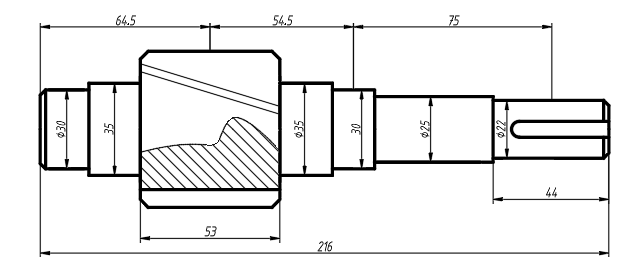
\includegraphics[width=1\textwidth]{pictures/shaft_II.png}
                    \caption{Phác thảo sơ bộ trục II}
                    \label{fig:shaft_II}
                \end{figure}
            \subsubsection{Phác thảo sơ bộ trục III}
               \begin{figure}[H]
                    \centering
                    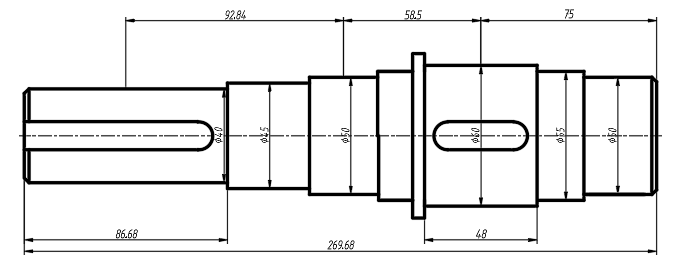
\includegraphics[width=1\textwidth]{pictures/shaft_III.png}
                    \caption{Phác thảo sơ bộ trục III}
                    \label{fig:shaft_III}
                \end{figure}
    \section{Thiết kế mối ghép then}
        \subsection{Tính mối ghép then}
            \begin{figure}[H]
                \centering
                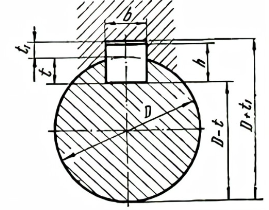
\includegraphics[width=0.4\textwidth]{pictures/key.png}
                \caption{Mối ghép then}
                \label{fig:key}
            \end{figure}
            \begin{itemize}
                \item Do các trục đều nằm trong hộp giảm tốc nên ta chọn then bằng. Để đảm bảo tính công nghệ, chọn then giống nhau trên cùng 1 trục.
                    \begin{figure}[H]
                        \centering
                        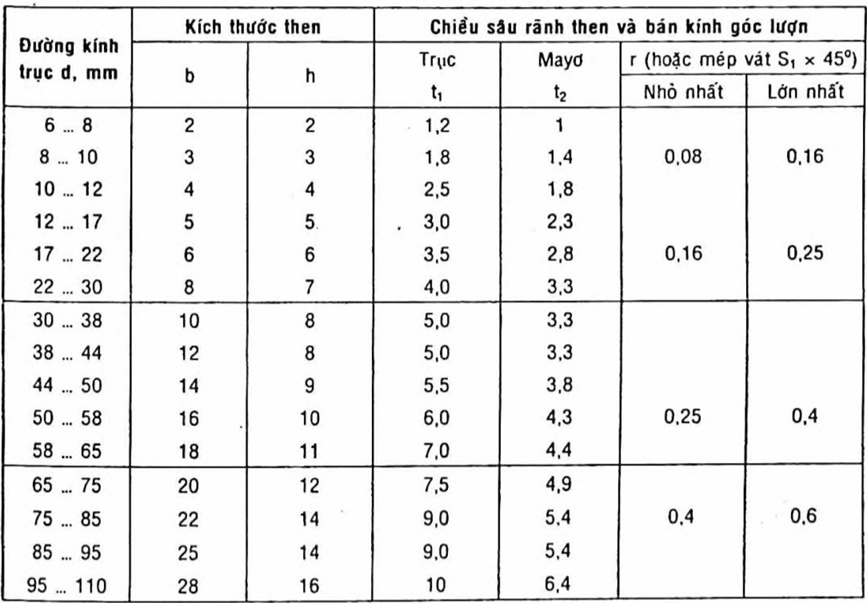
\includegraphics[width=0.8\textwidth]{pictures/key_standard.png}
                        \caption{Tiêu chuẩn về mối ghép then bằng}
                        \label{fig:key_standard}
                        \caption*{\footnotesize (Trích tài liệu \cite{btctm}, trang 188, phụ lục 13.1)}
                    \end{figure}
                \item Từ những dữ liệu tính toán được và bảng \ref{fig:key_standard} ta có bảng số liệu về then như sau:
                    \begin{table}[H]
                        \centering
                        \begin{tabular}{|c|c|c|c|c|}
                            \hline
                            \textbf{Tiết diện} & \textbf{d, mm} & \textbf{b x h, mm} & $\mathbf{t_{1}, mm}$ & $\mathbf{t_{2}, mm}$  \\
                            \hline
                            \textbf{Bánh đai bị dẫn} & 22 & 6 x 6 & 3.5 & 2.8  \\
                            \hline
                            \textbf{Bánh răng nghiêng (I)} & 40 & 12 x 8 & 5 & 3.3  \\
                            \hline
                            \textbf{Bánh răng nghiêng (II)} & 60 & 18 x 11 & 7 & 4.4  \\
                            \hline
                            \textbf{Bánh răng côn (I)} & 40 & 12 x 8 & 5 & 3.3  \\
                            \hline
                        \end{tabular}
                        \caption{Bảng số liệu về then}
                    \end{table}
            \end{itemize}

        \subsection{Kiểm nghiệm then}
            \begin{itemize}
                \item Xác định chiều dài các mayơ:
                    \begin{itemize}
                        \item Chiều dài mayơ bánh đai ở trục II:
                            \[
                                l_{m1} = B_{d} = 44 \, \mathrm{mm}
                            \]
                        \item Chiều dài mayơ bánh răng trụ răng nghiêng 1 ở trục II: 
                            \[
                                l_{m2} = B_{1}= 53 \, \mathrm{mm}
                            \]  
                        \item Chiều dài mayơ bánh răng trụ răng nghiêng 2 ở trục III:
                            \[
                                l_{m2} = B_{2}= 48 \, \mathrm{mm}
                            \]
                        \item Chiều dài mayơ bánh răng côn ở trục III:
                            \[
                                l_{m3} = B_{w}= 86.68 \, \mathrm{mm}
                            \]
                    \end{itemize}
                \item Xác định chiều dài then: 
                    \[
                        l_{t} = (0.8...0.9)l_m \footnote{Trích tài liệu \cite{tltk1}, trang 174.}
                    \]
                    \begin{itemize}
                        \item Chiều dài then bánh đai ở trục II:
                            \[
                                l_{t0} = (0.8...0.9)l_{m1} = (0.8...0.9) \cdot 44 = 35.2...39.6 \, \mathrm{mm}
                            \]
                            $\Rightarrow$ Theo tiêu chuẩn ta chọn $l_{t0} = 40 \, \mathrm{mm}$
                        \item Chiều dài then bánh răng trụ răng nghiêng 1 ở trục II: 
                            \[
                                l_{t1} = (0.8...0.9)l_{m2} = (0.8...0.9) \cdot 53 = 42.4...47.7 \, \mathrm{mm}
                            \]
                            $\Rightarrow$ Theo tiêu chuẩn ta chọn $l_{t1} = 45 \, \mathrm{mm}$
                        \item Chiều dài then bánh răng trụ răng nghiêng 2 ở trục III:
                            \[
                                l_{t2} = (0.8...0.9)l_{m2} = (0.8...0.9) \cdot 48  = 38.4...43.2  \, \mathrm{mm}
                            \]
                            $\Rightarrow$ Theo tiêu chuẩn ta chọn $l_{t2} = 40 \, \mathrm{mm}$
                        \item Chiều dài then bánh răng côn ở trục III:
                            \[
                                l_{t3} = (0.8...0.9)l_{m3} = (0.8...0.9) \cdot 86.68 = 69.34...78.01 \, \mathrm{mm}
                            \]
                            $\Rightarrow$ Theo tiêu chuẩn ta chọn $l_{t3} = 80 \, \mathrm{mm}$
                    \end{itemize}
                \item Kiểm tra then:
                    \begin{figure}[H]
                        \centering
                        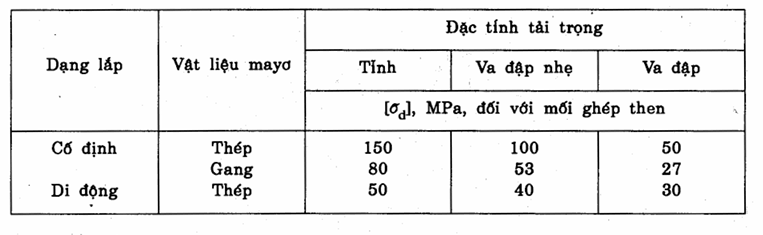
\includegraphics[width=0.8\textwidth]{pictures/key_check.png}
                        \caption{Ứng suất dập cho phép $\sigma_{d}$ đối với mối ghép then}
                        \caption*{\footnotesize (Trích tài liệu \cite{tltk1}, trang 178, bảng 9.5)}
                        \label{fig:key_check}
                    \end{figure}
                    \begin{itemize}
                        \item Do đặc tính tải trọng là tĩnh và dạng lắp là cố địng. Vật liệu mayơ làm bằng thép nên ứng suất dập cho phép $\sigma_{d} = 150 \, \mathrm{MPa}$.
                        \item Tính toán ứng suất dập:
                            \[
                                \sigma_{d} = \frac{2T \cdot 10^3}{t_{2} \cdot d \cdot l_{l}} \footnote{Trích tài liệu \cite{gtctm}, trang 623, công thức 16.1.}
                            \]
                            Trong đó: $l_{l} = l - b \, \mathrm{mm}$.
                        \item Ta có bảng số liệu về tính toán then:
                            \begin{table}[H]
                                \centering
                                \begin{tabular}{|c|c|c|c|c|c|}
                                    \hline
                                    \textbf{Tiết diện} & \textbf{d, mm} & \textbf{b x h x l, mm} & \textbf{T, Nm} & $\mathbf{t_{2}, mm}$ & $\mathbf{\sigma_{d}, MPa}$ \\
                                    \hline
                                    \textbf{Bánh đai bị dẫn} & 22 & 6 x 6 x 40  & 75.87 & 3.5 & 57.96  \\
                                    \hline
                                    \textbf{Bánh răng nghiêng (I)} & 40 & 12 x 8 x 45 & 75.87 & 5 & 22.99  \\
                                    \hline
                                    \textbf{Bánh răng nghiêng (II)} & 60 & 18 x 11 x 40 & 360.78 & 7 & 78.09  \\
                                    \hline
                                    \textbf{Bánh răng côn (I)} & 40 & 12 x 8 x 80 & 360.78 & 5 & 53.05 \\
                                    \hline
                                \end{tabular}
                                \caption{Bảng số liệu về then}
                            \end{table}
                            $\Rightarrow$ Điều kiện bền dập của cả 4 then đều thỏa mãn $\sigma_{d} < [\sigma_{d}]$. Then bằng được chọn theo tiêu chuẩn nên không cần thiết kiểm tra theo độ bền cắt.
                    \end{itemize}
                    \hspace*{0.6cm}Vì đường kính trục tại tiết diện lắp bánh răng nghiêng I là $40 (mm)$ và đường kính chân răng là $45.33 (mm)$. Khi đó khoảng cách từ đỉnh then đến chân răng $ = \frac{45.33 - 40}{2} - t_1 = -0.835 (mm)$ $\rightarrow$ Ta thiết kế bánh răng liền trục tại vị trí C và không lắp then.
            \end{itemize}
    \section{Kiểm nghiệm trục}
        \hspace*{0.6cm}Kết cấu trục vừa thiết kế đảm bảo được độ bền mỏi nếu hệ số an toàn tại các tiết diện nguy hiểm thỏa mãn điều kiện sau:
        $$s_j = \frac{s_{\sigma j}s_{\tau j}}{\sqrt{s^2_{\sigma j}+ s^2_{\tau j}}} \geq [s]$$
        Trong đó:
        \begin{itemize}
            \item[] $[s]$: Hệ số an toàn cho phép. Theo \textit{trang 195 tài liệu tham khảo \cite{tltk1}}, chọn $[s] = 3$ thì không cần kiểm nghiệm về độ cứng của trục.
            \item[] $s_{\sigma j}, s_{\tau j}$: Hệ số an toàn chỉ xét riêng ứng suất pháp và hệ số an toàn chỉ xét riêng ứng suất tiếp tại tiết diện j:
            \begin{align*}
                &s_{\sigma j} = \frac{\sigma_{-1}}{K_{\sigma dj}\sigma_{aj} + \psi_\sigma \sigma_{mj}} \\
                &s_{\tau j} = \frac{\tau_{-1}}{K_{\tau dj}\tau_{aj} + \psi_\tau \tau_{mj}}
            \end{align*}
            Trong đó:
            \begin{itemize}
                \item[--] $\sigma_{-1}, \tau_{-1}$: Giới hạn mỏi uốn và xoắn ứng với chu kỳ đối xứng.Theo \textit{trang 196 tài liệu tham khảo \cite{tltk1}}, lấy gần đúng $\sigma_{-1} = 0.436 \cdot \sigma_b = 0.436.850 = 370.6 (MPa)$ và $\tau_{-1} = 0.58 \cdot \sigma_{-1} = 0.58 \cdot 370.6 = 214.95 (MPa)$ vì vật liệu làm trục - Thép C45 là thép Carbon trung bình.
                \item[--] $\sigma_{aj}, \tau_{aj}, \sigma_{mj}, \tau_{mj}$: Biên độ và trị số trung bình của ứng suất pháp và ứng suất tiếp tại tiết diện j. Xét cho cả hai trục, ta đều có các tính chất sau:
                \begin{itemize}
                    \item[+] Đối với trục quay, ứng suất uốn thay đổi theo chu kỳ đối xứng:
                    $$\sigma_{mj} = 0; \sigma_{aj} = \frac{M_j}{W_j}$$
                    \item[+] Đối với trục quay 1 chiều, ứng suất xoắn tay đổi theo chu kỳ mạch động
                    $$\tau_{mj} = \tau_{aj} = \frac{T_j}{2W_{oj}}$$
                    Trong đó, $W_j, W_{oj}$ là momen cản uốn và momen cản xoắn tại tiết diện j của trục, được xác định theo \textit{bảng 10.6 tài liệu tham khảo \cite{tltk1}}. Vì trục II có 1 rãnh then và trục III có 2 rãnh then:
                    \begin{align*}
                        &W_{II} = \frac{\pi d_j^3}{32} - \frac{bt_1(d_j - t_1)^2}{2 \cdot d_j}\\
                        &W_{oII} = \frac{\pi d_j^3}{16} - \frac{bt_1(d_j - t_1)^2}{2 \cdot d_j}\\
                        &W_{III} = \frac{\pi d_j^3}{32} - \frac{bt_1(d_j - t_1)^2}{d_j}\\
                        &W_{oIII} = \frac{\pi d_j^3}{16} - \frac{bt_1(d_j - t_1)^2}{d_j}
                    \end{align*}
                \end{itemize}
                \item[--] $\psi_\sigma, \psi_\tau$: Hệ số kể đến ảnh hưởng của trị số ứng suất trung bình đến độ bền mỏi, theo \textit{bảng 10.7 tài liệu tham khảo [2]}. 
                \item[--] $K_{\sigma dj}, K_{\tau dj}$: Hệ số, được xác định theo:
                \begin{align*}
                    &K_{\sigma dj} = \frac{K_\sigma/\epsilon_\sigma + K_x - 1}{K_y}\\
                    &K_{\tau dj} = \frac{K_\tau/\epsilon_\tau + K_x - 1}{K_y}
                \end{align*}
                Trong đó:
                \begin{itemize}
                    \item[+] $K_x$: Hệ số tập trung ứng suất do trạng thái bề mặt, phụ thuộc vào phương pháp gia công và độ nhẵn bề mặt, cho trong \textit{bảng 10.8 tài liệu tham khảo \cite{tltk1}}.
                    \item[+] $K_y$: Hệ số tăng bền bề mặt trục, phụ thuộc vào phương pháp tăng bền bề mặt và cơ tính vật liệu, cho trong\textit{ bảng 10.9 tài liệu tham khảo \cite{tltk1}}.
                    \item[+] $\epsilon_\sigma, \epsilon_\tau$: Hệ số kích thước kể đến ảnh hưởng của kích thước tiết diện trục đến giới hạn mỏi, cho trong \textit{bảng 10.10 tài liệu tham khảo \cite{tltk1}}
                    \item[+] $K_\sigma, K_\tau$: Hệ số tập trung ứng suất thực tế khi uốn và khi xoắn, trị số của chúng phụ thuộc vào loại yếu tố gây tập trung ứng suất, cho trong \textit{bảng 10.11 tài liệu tham khảo \cite{tltk1}}.
                \end{itemize}
            \end{itemize}
    \end{itemize}
    \begin{table}[H]
        \centering
        \begin{tabular}{|c|c|c|}
            \hline
            \diagbox{\textbf{Thông số}}{\textbf{Trục}}  & \textbf{Trục II} & \textbf{Trục III} \\ \hline
            $\sigma_{-1} (\, \mathrm{MPa})$ & \multicolumn{2}{c|}{370.6}\\ \hline
            $\tau_{-1} (\, \mathrm{MPa})$ & \multicolumn{2}{c|}{214.95}\\ \hline
            $d$ & 40 & 55\\ \hline
            $b$ & 10 & 16 \\ \hline
            $t_1$ & 5 & 6 \\ \hline
            $\sigma_{mj} (\, \mathrm{MPa})$ & \multicolumn{2}{c|}{0} \\ \hline
            $\sigma_{aj} (\, \mathrm{MPa})$ & 22.09 & 85.81 \\ \hline
            $\tau_{mj} = \tau_{aj} (\, \mathrm{MPa})$ & 3.21 & 6.33 \\ \hline
            $W_j$ & 5517.56 & 12142.99 \\ \hline
            $W_{oj}$ & 11800.75 & 28476.82\\ \hline
            $M (\, \mathrm{N.mm})$ & 121914.81 & 1041993.85 \\ \hline
            $T (\, \mathrm{N.mm})$ & 75870 & 360780 \\ \hline
            $\psi_{\sigma}$ &  \multicolumn{2}{c|}{$0.1$} \\ \hline
            $\psi_{\tau}$ &  \multicolumn{2}{c|}{$0.05$} \\ \hline
            $K_{x}$ & \multicolumn{2}{c|}{1} \\ \hline
            $K_{y}$ &  \multicolumn{2}{c|}{2.5} \\ \hline
            $\epsilon_\sigma$ & 0.85 & 0.8 \\ \hline
            $\epsilon_\tau$ & 0.78 & 0.75 \\ \hline
            $K_{\sigma}$ & \multicolumn{2}{c|}{$2.07$} \\ \hline
            $K_{\tau}$ & \multicolumn{2}{c|}{$1.97$} \\ \hline
            $K_{\sigma dj}$ & 0.974 & 1.04 \\ \hline
            $K_{\tau dj}$ & 1.01 & 1.05 \\ \hline
            $s_{\sigma j}$ & 17.22 & 4.15 \\ \hline
            $s_{\tau j}$ & 63.17 & 30.87 \\ \hline
            $s_j$ & 16.61 & 4.11 \\ \hline
        \end{tabular}
        \caption{Bảng thông số bộ truyền bánh răng trụ răng nghiêng}
    \end{table}
    $\rightarrow$ Cả hai trục đều đảm bảo được độ bền mỏi, không cần kiểm nghiệm về độ bền cứng.
    
                    
            
            